\chapterimage{./Images/head2.jpg} % Chapter heading image
\chapter{The Introduction}
\section{Administrative Information}
\begin{itemize}
    \item Pre-labs
    \item use the CPUlator website
    \item We use NIOS V (variant of RISC-V)
\end{itemize}

\section{Computers}
\subsection*{What does a processor do?}
\begin{itemize}
    \item Data Calculations

    \item Data Movement
\end{itemize}

\subsection*{What does a memory do?}
\begin{figure}[h]
    \centering
    \begin{tikzpicture}
        \node[draw, rectangle] (a) at (0,0) {Processor};
        \node[draw, rectangle] (b) at (6,0) {Memory};
        \node[draw] (c) at (3,-2) {Interconected};
        \node[draw, rectangle] (d) at (3,-4) {I/O};
        \draw[->] (a) -- (c);
        \draw[->] (b) -- (c);
        \draw[->] (c) -- (d);
    \end{tikzpicture}
\end{figure}

\begin{definition}
    [Actuator]
    A device that converts an electrical signal into a physical action.
\end{definition}

\begin{definition}
    [Sensor]
    A device that converts a physical action into an electrical signal.
\end{definition}

\section{Bit Representation}
\begin{definition}
    [Overflow]
    When the result of an operation is too large to be represented in the number of bits available.
\end{definition}

\subsection*{C Programming integer bit-size assignments}
\begin{itemize}
    \item \texttt{unsigned char} is 8 bits
    \item \texttt{int} is 32 bits
    \item \texttt{long} is 64 bits
    \item \texttt{long long} is 64 bits
\end{itemize}

\begin{definition}
    [Signed Integers]
    The most significant bit (Furthest left) is the sign bit. 0 is positive, 1 is negative. \\
    Unoften used.
\end{definition}

\begin{definition}
    [2's Complement]
    A way to represent negative numbers in binary. \\
    This is the most common way to represent negative numbers in binary.
\end{definition}

\begin{figure}[h]
    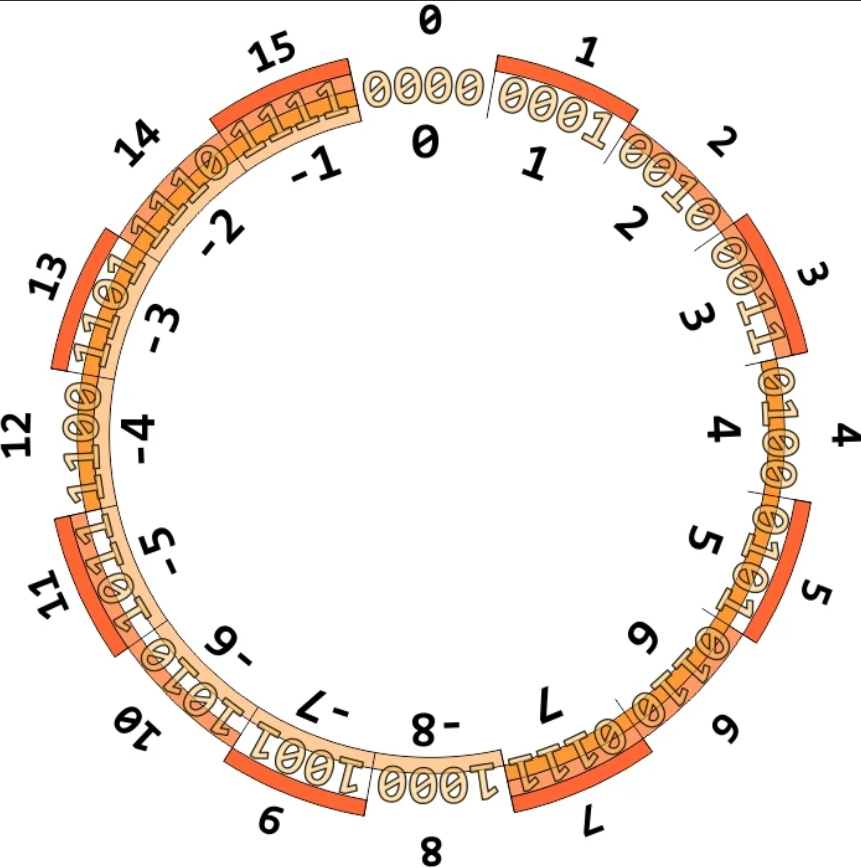
\includegraphics[width=0.5\textwidth]{./LECTURE_1/TwosComplement.png}
    \centering
    \caption[short]{2's Complement of 4 bits}
\end{figure}
